\documentclass[tikz,border=0.1in]{standalone}
\usepackage{tikz}
\usetikzlibrary{positioning, arrows.meta, fit, backgrounds, calc}
\usepackage[T1]{fontenc}
\usepackage{amssymb}
\usepackage[scaled=0.95]{helvet}
\renewcommand{\familydefault}{\sfdefault}

\definecolor{miamired}{HTML}{C3142D}
\definecolor{agentblue}{HTML}{1D5FAD}
\definecolor{evalgold}{HTML}{EFDB72}
\definecolor{nonfund}{HTML}{CCC9B8}

\tikzset{
  colhead/.style = {rectangle, rounded corners, ultra thick, align=center,
                    text width=7.6cm, minimum height=0.95cm,
                    font=\small\bfseries, inner sep=5pt},
  item/.style    = {rectangle, rounded corners, draw=gray!50, thick,
                    fill=white, align=left, text width=7.6cm,
                    font=\small, inner sep=6pt},
  lab/.style     = {font=\small, align=center},
}

\begin{document}
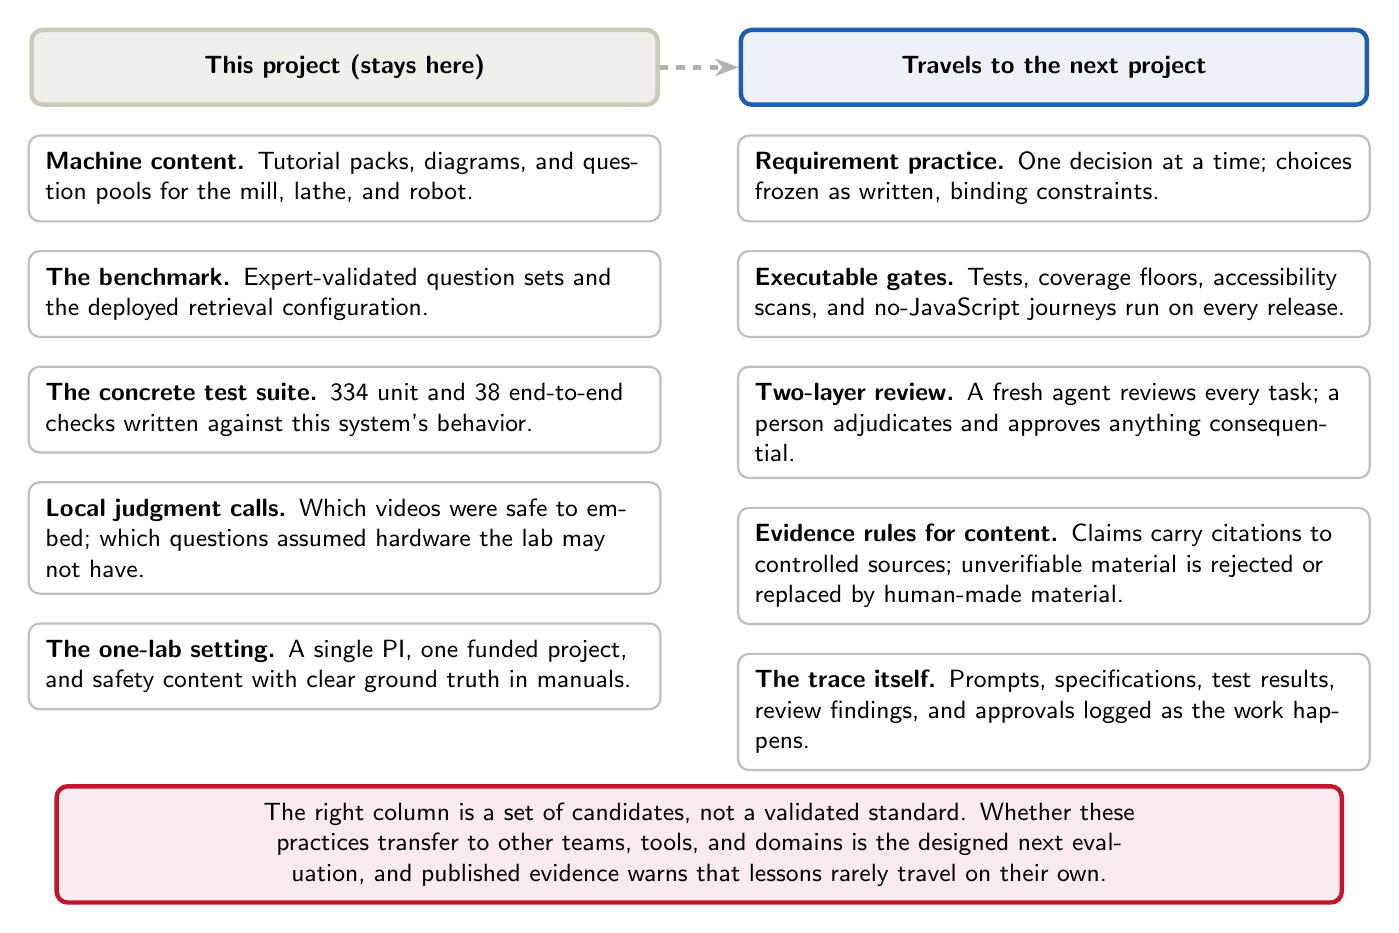
\begin{tikzpicture}[node distance=0.35cm and 1.0cm]

% Column heads: this project on the left, what follows on the right
\node (h1) [colhead, draw=nonfund, fill=nonfund!30] {This project (stays here)};
\node (h2) [colhead, draw=agentblue, fill=agentblue!8, right=of h1] {Travels to the next project};
\draw [ultra thick, -{Stealth[length=3mm]}, draw=gray!60, dashed] (h1) -- (h2);

% Case-specific column (left)
\node (b1) [item, below=of h1] {\textbf{Machine content.} Tutorial packs, diagrams, and question pools for the mill, lathe, and robot.};
\node (b2) [item, below=of b1] {\textbf{The benchmark.} Expert-validated question sets and the deployed retrieval configuration.};
\node (b3) [item, below=of b2] {\textbf{The concrete test suite.} 334 unit and 38 end-to-end checks written against this system's behavior.};
\node (b4) [item, below=of b3] {\textbf{Local judgment calls.} Which videos were safe to embed; which questions assumed hardware the lab may not have.};
\node (b5) [item, below=of b4] {\textbf{The one-lab setting.} A single PI, one funded project, and safety content with clear ground truth in manuals.};

% Reusable column (right)
\node (a1) [item, below=of h2] {\textbf{Requirement practice.} One decision at a time; choices frozen as written, binding constraints.};
\node (a2) [item, below=of a1] {\textbf{Executable gates.} Tests, coverage floors, accessibility scans, and no-JavaScript journeys run on every release.};
\node (a3) [item, below=of a2] {\textbf{Two-layer review.} A fresh agent reviews every task; a person adjudicates and approves anything consequential.};
\node (a4) [item, below=of a3] {\textbf{Evidence rules for content.} Claims carry citations to controlled sources; unverifiable material is rejected or replaced by human-made material.};
\node (a5) [item, below=of a4] {\textbf{The trace itself.} Prompts, specifications, test results, review findings, and approvals logged as the work happens.};

% Caveat band
\node (band) [lab, below=0.55cm of $(a5.south)!0.5!(b5.south)$, text width=15.9cm,
  draw=miamired, ultra thick, fill=miamired!8, rounded corners, inner sep=6pt] {%
  The right column is a set of candidates, not a validated standard. Whether these
  practices transfer to other teams, tools, and domains is the designed next
  evaluation, and published evidence warns that lessons rarely travel on their own.};

\end{tikzpicture}
\end{document}
